% 通用模板：基于学校的版式抽取结果生成
\documentclass[UTF8,a4paper,zihao=-4]{ctexart}
% Common preamble and formatting commands for the JXUST LaTeX template.
\usepackage{geometry}
\geometry{
  top=2.54cm,
  bottom=2.54cm,
  left=3.18cm,
  right=3.18cm,
  headheight=14pt,
  headsep=0.8cm,
  footskip=1.0cm
}

\usepackage{fontspec}
\usepackage{graphicx}
\usepackage{caption}
\usepackage{array}
\usepackage{booktabs}
\usepackage{tabularx}
\usepackage{fancyhdr}
\usepackage{hyperref}
\usepackage{bookmark}

\setmainfont{Times New Roman}
\setCJKmainfont{SimSun}
\setCJKsansfont{SimHei}
\setmonofont{Courier New}

\newcommand{\wordmainfont}{\fontsize{12pt}{20pt}\selectfont}
\AtBeginDocument{\wordmainfont}

\setlength{\parindent}{0pt}
\setlength{\parskip}{0pt}

\hypersetup{
  unicode=true,
  pdfpagelabels=true,
  bookmarksopen=true,
  bookmarksopenlevel=2
}

\pagestyle{fancy}
\fancyhf{}
\fancyhead[C]{江西理工大学2026届本科毕业设计（论文）}
\fancyfoot[C]{\thepage}
\renewcommand{\headrulewidth}{0.4pt}
\renewcommand{\footrulewidth}{0pt}

\captionsetup{font=small,labelsep=space}

\newcounter{bookmarkchapter}
\newcounter{bookmarksection}[bookmarkchapter]
\newcounter{bookmarksubsection}[bookmarksection]

\newcommand{\chaptertitle}[1]{%
  \refstepcounter{bookmarkchapter}%
  \setcounter{bookmarksection}{0}%
  \setcounter{bookmarksubsection}{0}%
  \pdfbookmark[0]{#1}{bk-ch-\thebookmarkchapter}%
  \begin{center}
    \heiti\zihao{3} #1
  \end{center}
  \vspace{0.8\baselineskip}
}

\newcommand{\sectiontitle}[1]{%
  \refstepcounter{bookmarksection}%
  \setcounter{bookmarksubsection}{0}%
  \pdfbookmark[1]{#1}{bk-sec-\thebookmarkchapter-\thebookmarksection}%
  \vspace{0.6\baselineskip}
  \noindent{\heiti\zihao{4} #1}\par
  \vspace{0.3\baselineskip}
}

\newcommand{\subsectiontitle}[1]{%
  \refstepcounter{bookmarksubsection}%
  \pdfbookmark[2]{#1}{bk-sub-\thebookmarkchapter-\thebookmarksection-\thebookmarksubsection}%
  \vspace{0.4\baselineskip}
  \noindent{\heiti\zihao{-4} #1}\par
  \vspace{0.2\baselineskip}
}

\newcommand{\cnabstractpara}[1]{%
  {\wordmainfont\setlength{\parindent}{2em}\indent #1\par}
}

\newcommand{\enabstractpara}[1]{%
  {\wordmainfont\setlength{\parindent}{4em}\indent #1\par}
}

\newcommand{\cnkeywordline}[1]{%
  {\wordmainfont\noindent{\heiti 关键词：}#1\par}
}

\newcommand{\enkeywordline}[1]{%
  {\wordmainfont\noindent{\bfseries Keywords:} #1\par}
}

\newcommand{\bodypara}[1]{%
  {\wordmainfont\setlength{\parindent}{2em}\indent #1\par}
}

\newcommand{\firstbodypara}[1]{%
  \par\addvspace{9pt}%
  {\wordmainfont\setlength{\parindent}{2em}\indent #1\par}
}

\newcommand{\compactpara}[1]{%
  \par\addvspace{3pt}%
  {\wordmainfont\noindent #1\par}%
  \addvspace{3pt}
}

\newenvironment{wordreferences}{\par}{\par}

\newcommand{\referenceentry}[2]{%
  {\wordmainfont\noindent[#1]\quad #2\par}
}

\newcommand{\placeholderfigurebox}[1]{%
  \fbox{\parbox[c][0.22\textheight][c]{0.72\textwidth}{\centering #1}}
}

\newcommand{\placeholdertablebox}[1]{%
  \fbox{\parbox[c][0.15\textheight][c]{0.78\textwidth}{\centering #1}}
}

\newcolumntype{Y}{>{\centering\arraybackslash}X}

\newcommand{\equationplaceholder}[1]{%
  \begin{center}
    \fbox{\parbox{0.82\textwidth}{\centering #1}}
  \end{center}
}


\begin{document}
\pagenumbering{Roman}

\chaptertitle{摘  要}
\cnabstractpara{这里填写中文摘要内容。}
\cnkeywordline{气动位置伺服系统；无杆气缸；模型预测控制；轨迹跟踪}

\clearpage
\chaptertitle{ABSTRACT}
\enabstractpara{Write the English abstract here.}
\enkeywordline{Pneumatic position servo system; rodless cylinder; model predictive control; trajectory tracking}

\clearpage
\pagenumbering{arabic}
\chaptertitle{第一章 绪论}
\sectiontitle{1.1 研究背景及意义}
\subsectiontitle{1.1.1 研究背景}
\firstbodypara{这里填写章节首段正文。}
\subsectiontitle{1.1.2 研究意义}
\bodypara{这里填写普通正文。}

\sectiontitle{1.2 国内外研究现状}
\bodypara{这里填写综述内容。}

\sectiontitle{1.3 本文研究内容及安排}
\compactpara{这里填写紧凑参数或条目型内容。}
\bodypara{这里填写研究内容概述。}

\begin{figure}[htbp]
\centering
\IfFileExists{figures/image2.png}{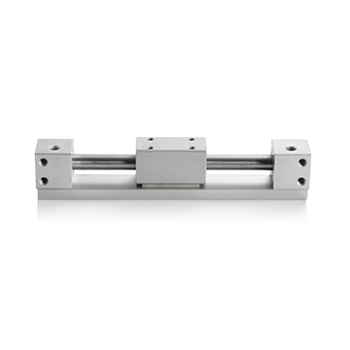
\includegraphics[width=0.58\textwidth]{figures/image2.png}}{\placeholderfigurebox{图像占位示例}}
\caption{图 1-1 示例图片题注}
\end{figure}

\begin{table}[htbp]
\centering
\caption{表 1-1 示例表格题注}
\renewcommand{\arraystretch}{1.2}
\begin{tabularx}{\textwidth}{@{}YYY@{}}
\toprule
项目 & 指标 & 说明 \\
\midrule
示例A & 数值1 & 说明文字 \\
示例B & 数值2 & 说明文字 \\
\bottomrule
\end{tabularx}
\end{table}

\begin{equation}
a^2 + b^2 = c^2
\end{equation}

\clearpage
\chaptertitle{参考文献}
\begin{wordreferences}
\referenceentry{1}{作者. 文献题名[J]. 期刊名, 年份, 卷(期): 页码.}
\end{wordreferences}

\clearpage
\chaptertitle{致  谢}
\bodypara{这里填写致谢内容。}

\end{document}
